\chapter{介绍}
	在数据中查找模式的问题是一个基础性问题,并且有很长而成功的历史。例如,Tycho Brahe在16世纪广泛的天文观察是的开普勒发现了天体运动规律,这又提供了经典力学发展的跳板。同样的,原子光谱规律的发现也对量子物理的发展和验证起到了关键的作用。模式识别领域关注于使用计算机算法来自动地发现数据中的规律,并且使用这些规律进行如对不同类别进行分类的一些活动。
	
	思考手写数字的识别例子,如图1.1。每个数字对应$28 \times 28$个像素,可以使用包含784个实数的向量$\mathbf{x}$来表示。目标是去构建一个机器,向量$\mathbf{x}$作为输入,产生数字$0,\dots, 9$作为输出。可以使用手工规则或者启发式来根据笔画形状来区分数字,但是这种方法在实践中会导致增加例外的规则,并且不约而同地给出糟糕的结果。
	
\begin{figure}
	\centering
	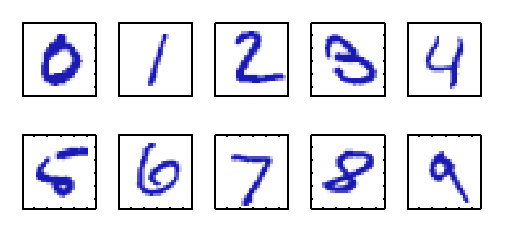
\includegraphics[width=8cm]{Figure1-1.eps}
	\caption{Examples of hand-written digits taken from US zip codes} 
	\label{fig:endb-flow} 
\end{figure}

	更优的结果是采用机器学习方法,这种方法中有一个很大的数字集合 $N\{\lstset{breaklines} \mathbf{x_1}, \dots, x_N \}$ 称为训练集,用来训练得到可适应模型的参数。
\section{图模型}

